% ============================================================
%  Projeto Integrativo 3 — Projeto 3, entrega Q1: apresentação
%  Detecção de quedas no vestível: modelos, pipeline e o Random Forest
%  Escola Politécnica da USP
%
%  figuras/, tabelas/ e numeros.tex são gerados por
%  modelo/experimentos/10_figuras_apresentacao.py (nenhum número é digitado à mão).
%  Compile com `pdflatex main.tex`, duas vezes. Roteiro da fala: ../roteiro-apresentacao.md
% ============================================================
\documentclass[aspectratio=169,10pt]{beamer}

\usepackage[utf8]{inputenc}
\usepackage[T1]{fontenc}
\usepackage[brazilian]{babel}
\usepackage{lmodern}
\usepackage{amsmath,amssymb}
\usepackage{booktabs,makecell,array}
\usepackage{graphicx}
\usepackage{tikz}
\usetikzlibrary{arrows.meta,positioning,calc}

% GERADO por modelo/experimentos/10_figuras_apresentacao.py: não edite à mão.

\newcommand{\nPessoas}{38}
\newcommand{\nEnsaios}{4\,505}
\newcommand{\nEnsaiosQueda}{1\,798}
\newcommand{\nEnsaiosAtividade}{2\,707}
\newcommand{\horasAtividade}{14,5}
\newcommand{\nProprios}{18}
\newcommand{\nPropriosQueda}{10}
\newcommand{\nPropriosAtividade}{8}
\newcommand{\lOn}{2,0}
\newcommand{\gatilhoPassam}{99,2}
\newcommand{\disparosPicos}{858}
\newcommand{\disparosCausal}{753}
\newcommand{\nJanelas}{12\,723}
\newcommand{\nImpactos}{1\,784}
\newcommand{\nAtributos}{23}
\newcommand{\nJanelasAtividade}{10\,939}
\newcommand{\picoBruto}{10,1}
\newcommand{\picoFiltrado}{7,6}
\newcommand{\exDisparos}{6}
\newcommand{\exQuedaLivre}{0,35}
\newcommand{\exPico}{7,6}
\newcommand{\exInclinacao}{90}
\newcommand{\exPosStd}{0,035}
\newcommand{\rfRelAlarmesA}{0,4}
\newcommand{\rfRelSensA}{95,7}
\newcommand{\rfRelAlarmesB}{0,8}
\newcommand{\rfRelSensB}{94,4}
\newcommand{\arvoreAlarmesA}{5,3}
\newcommand{\lrRelAlarmesA}{1,4}
\newcommand{\knnMB}{1,6}
\newcommand{\soTempo}{95,4}
\newcommand{\soFFT}{7,8}
\newcommand{\soAR}{5,2}
\newcommand{\rfPropriosQuedas}{7}
\newcommand{\rfPropriosAlarmes}{0}
\newcommand{\rfVestAlarmes}{0,55}
\newcommand{\rfVestSens}{95,1}
\newcommand{\rfVestLimiar}{0,73}
\newcommand{\rfVestNos}{8\,854}
\newcommand{\rfVestKB}{104}
\newcommand{\lrVestAlarmes}{0,62}
\newcommand{\nVetores}{26}
\newcommand{\nTrechos}{8}
\newcommand{\funilDetectadas}{1\,695}
\newcommand{\funilDetectadasPct}{94,3}
\newcommand{\funilPassam}{1\,784}
\newcommand{\giniAtributo}{inclinação}
\newcommand{\giniLimiar}{36,1}
\newcommand{\giniUnidade}{$^\circ$}
\newcommand{\giniPai}{0,50}
\newcommand{\giniEsq}{0,04}
\newcommand{\giniDir}{0,04}
\newcommand{\giniGanho}{0,46}
\newcommand{\giniQuedasEsq}{37}
\newcommand{\giniAtivEsq}{10\,707}
\newcommand{\giniQuedasDir}{1\,747}
\newcommand{\giniAtivDir}{232}
\newcommand{\pesoQueda}{3,57}
\newcommand{\pesoAtividade}{0,58}
\newcommand{\atributosPorNo}{4}
\newcommand{\impPrimeiro}{mudança de inclinação}
\newcommand{\impSegundo}{assimetria de $|a|$}
\newcommand{\votoQueda}{0,86}
\newcommand{\votoCorrida}{0,00}
\newcommand{\votoDificil}{0,58}
\newcommand{\votoDificilCodigo}{D11}
\newcommand{\votoDificilNome}{tentar levantar e desabar na cadeira}


% --- Cores (as do relatório e as das figuras) ---
\definecolor{uspblue}{RGB}{0,84,166}
\definecolor{lightblue}{RGB}{220,235,248}
\definecolor{queda}{HTML}{EB6834}
\definecolor{atividade}{HTML}{2A78D6}
\definecolor{tinta}{HTML}{0B0B0B}
\definecolor{tinta2}{HTML}{52514E}
\definecolor{mudo}{HTML}{898781}

% --- Tema próprio, simples ---
\setbeamercolor{structure}{fg=uspblue}
\setbeamercolor{normal text}{fg=tinta}
\setbeamercolor{alerted text}{fg=queda}
\setbeamercolor{frametitle}{fg=white,bg=uspblue}
\setbeamercolor{block title}{fg=white,bg=uspblue}
\setbeamercolor{block body}{bg=lightblue}
\setbeamerfont{frametitle}{size=\large,series=\bfseries}
\setbeamertemplate{navigation symbols}{}
\setbeamertemplate{itemize items}[circle]
\setbeamertemplate{itemize subitem}[triangle]
\setbeamertemplate{enumerate items}[default]
\setbeamertemplate{blocks}[rounded][shadow=false]
\setbeamertemplate{frametitle}{%
  \nointerlineskip
  \begin{beamercolorbox}[wd=\paperwidth,ht=3.6ex,dp=1.4ex,leftskip=0.6cm,rightskip=0.6cm]{frametitle}%
    \usebeamerfont{frametitle}\insertframetitle
  \end{beamercolorbox}%
  \vspace{0.05cm}
}
\setbeamertemplate{footline}{%
  \leavevmode
  \begin{beamercolorbox}[wd=\paperwidth,ht=2.4ex,dp=1.1ex,leftskip=0.6cm,rightskip=0.6cm]{normal text}%
    \tiny\color{mudo}EPUSP -- Projeto Integrativo 3 \,$\cdot$\, Projeto 3, entrega Q1 \,$\cdot$\,
    Detecção de quedas no vestível\hfill\insertframenumber/\inserttotalframenumber
  \end{beamercolorbox}}
\setlength{\leftmargini}{1.1em}
\setlength{\leftmarginii}{1.1em}
\setbeamersize{text margin left=0.6cm, text margin right=0.6cm}

% --- Macros ---
\newcommand{\amag}{|a|}
\newcommand{\wmag}{|\omega|}
\newcommand{\nota}[1]{{\footnotesize\color{tinta2}#1}}
\newcommand{\figura}[1]{\begin{center}\includegraphics[width=\linewidth]{figuras/#1}\end{center}}

\tikzset{
  bloco/.style={draw=uspblue, line width=0.8pt, rounded corners=3pt, fill=white, align=center,
                font=\scriptsize, minimum height=1.25cm, text width=1.6cm, inner sep=3pt},
  destaque/.style={bloco, fill=lightblue},
  seta/.style={-{Stealth[length=2.2mm]}, line width=0.9pt, color=uspblue},
  setafina/.style={-{Stealth[length=1.8mm]}, line width=0.6pt, color=tinta2},
  rotulo/.style={font=\tiny, color=tinta2, align=center},
}

\begin{document}

% ============================================================
%  Capa
% ============================================================
\begin{frame}[plain]
  \centering
  \vspace{0.15cm}
  
\includegraphics[height=1.5cm]{imagens/Logo-Escola-Politecnica.jpg}\\[0.15cm]
  {\footnotesize\bfseries UNIVERSIDADE DE S\~AO PAULO \,--\, ESCOLA POLIT\'ECNICA}\\[0.4cm]
  {\color{uspblue}\rule{0.82\paperwidth}{1.2pt}}\\[0.3cm]
  {\LARGE\bfseries\color{uspblue} Detecção de quedas no vestível}\\[0.25cm]
  {\large Modelos testados, o pipeline e o Random Forest escolhido}\\[0.25cm]
  {\color{uspblue}\rule{0.82\paperwidth}{1.2pt}}\\[0.4cm]
  {\small Projeto Integrativo 3 \,--\, Projeto 3, entrega Q1}\\[0.4cm]
  {\footnotesize
   \begin{tabular}{l@{\hspace{0.8cm}}l@{\hspace{0.8cm}}l}
     Dimitri Garcia & Henrique Guimarães Margarido & Henrique Santiago \\
     \color{tinta2}NUSP 1682224 & \color{tinta2}NUSP 5797753 & \color{tinta2}NUSP 16872729 \\
   \end{tabular}}\\[0.35cm]
  {\scriptsize\color{tinta2} Novembro de 2026}
\end{frame}

% ============================================================
%  Objetivo e dados
% ============================================================
\begin{frame}{Objetivo: identificar as quedas}
  \begin{columns}[T,onlytextwidth]
    \begin{column}{0.56\textwidth}
      \begin{itemize}
        \item Reconhecer, \textbf{na própria pulseira}, quando o idoso cai, a partir do acelerômetro e do giroscópio
              do MPU-6050 (6 eixos a 200\,Hz) e processando no ESP32-S3.
        \item A queda detectada segue para o hub do quarto e para a central, que avisa o cuidador.
        \item A resposta é \textbf{binária}: \alert{queda} ou \textcolor{atividade}{não queda}.\\
              \nota{Os 15 tipos de queda e as 19 atividades servem para entender os erros, não como classes.}
        \item Duas metas, que puxam em sentidos opostos:
          \begin{itemize}
            \item detectar \textbf{quase todas as quedas};
            \item quase \textbf{nunca dar alarme falso} no dia a dia: andar, correr, sentar\ldots
          \end{itemize}
      \end{itemize}
    \end{column}
    \begin{column}{0.4\textwidth}
      \vspace{0.2cm}
      \centering
      \begin{tikzpicture}[node distance=0.5cm]
        \node[destaque, text width=3.6cm, minimum height=1cm] (s) {\small 6 sinais do vestível\\[-1pt]
              \tiny $a_x, a_y, a_z$ (g) \;$\cdot$\; $\omega_x, \omega_y, \omega_z$ ($^\circ$/s)};
        \node[bloco, text width=3.6cm, minimum height=0.85cm, below=of s] (m) {\small modelo};
        \node[bloco, text width=1.55cm, minimum height=0.7cm, below left=0.55cm and -1.6cm of m,
              draw=queda, fill=queda!12] (q) {\small\bfseries\color{queda} queda};
        \node[bloco, text width=1.55cm, minimum height=0.7cm, below right=0.55cm and -1.6cm of m,
              draw=atividade, fill=atividade!10] (n) {\small\bfseries\color{atividade} não queda};
        \draw[seta] (s) -- (m);
        \draw[seta] (m) -- (q);
        \draw[seta] (m) -- (n);
      \end{tikzpicture}\\[0.3cm]
      \nota{As metas viram duas medidas: \textbf{quedas detectadas (\%)} e \textbf{alarmes falsos por hora} de
            atividade.}
    \end{column}
  \end{columns}
\end{frame}

\begin{frame}{Os dados: a base pública SisFall}
  \figura{ap_dados.png}
  \vspace{-0.25cm}
  \begin{columns}[T,onlytextwidth]
    \begin{column}{0.49\textwidth}
      \begin{itemize}
        \item \textbf{\nPessoas{} pessoas} (23 jovens e 15 idosos) e \textbf{\nEnsaios{} ensaios}, com o sensor na
              \textbf{cintura}, a 200\,Hz.
        \item \nEnsaiosQueda{} quedas de 15 tipos (escorregão, tropeço, desmaio, ao sentar\ldots), em colchão.
      \end{itemize}
    \end{column}
    \begin{column}{0.49\textwidth}
      \begin{itemize}
        \item \nEnsaiosAtividade{} atividades de 19 tipos, somando \horasAtividade\,h: andar, correr, escada, sentar,
              deitar, pular.
        \item Correr e sentar rápido também têm picos altos: \textbf{o pico sozinho não decide}.
      \end{itemize}
    \end{column}
  \end{columns}
\end{frame}

\begin{frame}{Os dados: os nossos ensaios e a faixa do sensor}
  \figura{ap_saturacao.png}
  \vspace{-0.25cm}
  \begin{columns}[T,onlytextwidth]
    \begin{column}{0.49\textwidth}
      \begin{itemize}
        \item \textbf{\nProprios{} ensaios nossos}: \nPropriosQueda{} quedas (frente, costas, joelhos) e
              \nPropriosAtividade{} de andar e correr; uma pessoa, na cintura.
        \item Gravados em $\pm$2\,g: \textbf{saturam}, e o $\amag$ não passa de $2\sqrt{3}\approx 3{,}46$\,g.
      \end{itemize}
    \end{column}
    \begin{column}{0.49\textwidth}
      \begin{itemize}
        \item Dois cenários, saturando a SisFall: \textbf{A}, $\pm$8\,g (o vestível); \textbf{B}, $\pm$2\,g (os
              nossos ensaios).
        \item Treino e avaliação na SisFall; os nossos ensaios são um \textbf{teste externo}.
      \end{itemize}
    \end{column}
  \end{columns}
\end{frame}

% ============================================================
%  Pipeline
% ============================================================
\begin{frame}{O pipeline}
  \vspace{0.3cm}
  \centering
  \begin{tikzpicture}[node distance=0.26cm]
    \node[bloco] (sensor) {\textbf{Sensor}\\MPU-6050\\6 eixos, 200\,Hz};
    \node[bloco, right=of sensor] (filtro) {\textbf{1. Filtro}\\passa-baixa\\20\,Hz};
    \node[bloco, right=of filtro] (gatilho) {\textbf{2. Gatilho}\\pico de $\amag$\\$\ge$ \lOn\,g};
    \node[bloco, right=of gatilho] (janela) {\textbf{3. Janela}\\$-$1,0\,s a\\+0,8\,s};
    \node[bloco, right=of janela] (atrib) {\textbf{4. Atributos}\\\nAtributos{} números\\por janela};
    \node[destaque, right=of atrib, text width=1.95cm] (clf) {\textbf{5. Classificador}\\Random\\Forest};
    \node[bloco, right=of clf, draw=queda] (dec) {\textbf{6. Decisão}\\$P(\text{queda})$\\$\ge$ \rfVestLimiar};
    \foreach \a/\b in {sensor/filtro, filtro/gatilho, gatilho/janela, janela/atrib, atrib/clf, clf/dec}
      \draw[seta] (\a) -- (\b);
    \node[rotulo, below=0.15cm of filtro] {tira ruído\\e vibração};
    \node[rotulo, below=0.15cm of gatilho] {acorda o\\classificador};
    \node[rotulo, below=0.15cm of janela] {antes, impacto\\e depois};
    \node[rotulo, below=0.15cm of atrib] {queda livre,\\quietude, inclinação};
    \node[rotulo, below=0.15cm of clf] {só roda quando\\o gatilho dispara};
    \node[rotulo, below=0.15cm of dec] {depois, 30\,s\\sem novo alarme};
  \end{tikzpicture}

  \vspace{0.55cm}
  \begin{itemize}
    \item O \textbf{gatilho} é um limiar simples: deixa passar quase todas as quedas, mas também dispara ao correr ou
          sentar com força. Ele \textbf{não decide}; só diz \emph{quando} vale a pena olhar.
    \item Quem decide é o \textbf{classificador}, que olha a janela inteira: antes, no impacto e depois.
    \item Tudo roda amostra a amostra no ESP32-S3 do vestível.
  \end{itemize}
\end{frame}

\begin{frame}{2. Gatilho: o limiar vira um passo do pipeline}
  \begin{columns}[T,onlytextwidth]
    \begin{column}{0.5\textwidth}
      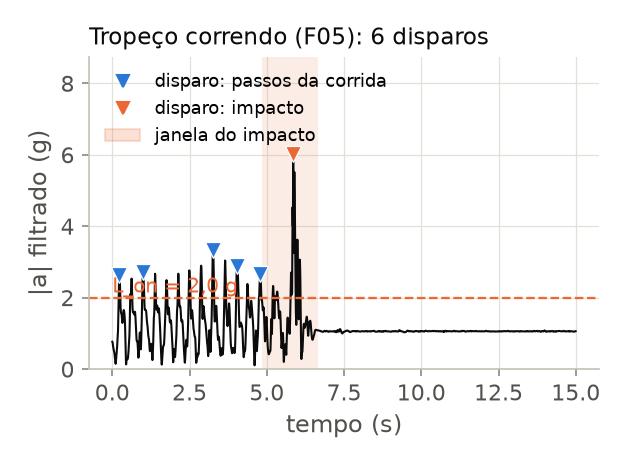
\includegraphics[width=\linewidth]{figuras/ap_gatilho_exemplo.png}
    \end{column}
    \begin{column}{0.5\textwidth}
      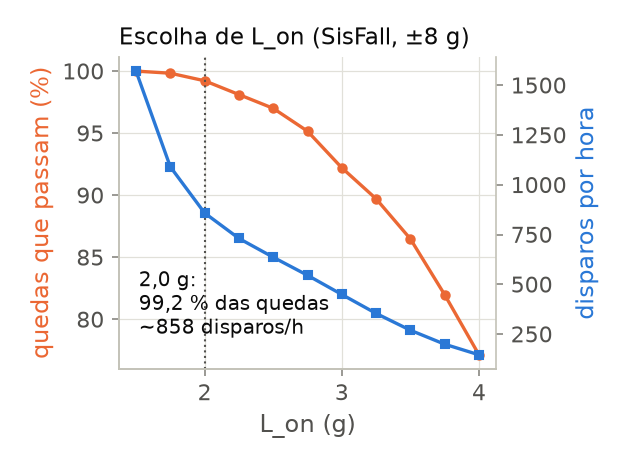
\includegraphics[width=\linewidth]{figuras/ap_gatilho_curva.png}
    \end{column}
  \end{columns}
  \vspace{0.05cm}
  \begin{itemize}
    \item Dispara num \textbf{pico de $\amag$ filtrado $\ge$ \lOn\,g}; o pico só vale depois de 0,5\,s sem um valor
          maior. Num tropeço correndo, cada passo dispara (\exDisparos{} disparos); só o impacto é queda.
    \item \lOn\,g é o maior limiar que ainda deixa passar \textbf{\gatilhoPassam\,\% das quedas}. O preço: o
          classificador acorda $\sim$\disparosPicos{} vezes por hora de atividade.
  \end{itemize}
\end{frame}

\begin{frame}{3 e 4. A janela e os atributos}
  \figura{ap_janela.png}
  \vspace{-0.35cm}
  {\footnotesize
  \textbf{Janela:} 1,0\,s antes e 0,8\,s depois do pico. \textbf{\nAtributos{} atributos no tempo}, independentes de
  como a pulseira está presa: momentos de $\amag$ (média, RMS, desvio, extremos, crista, curtose, assimetria,
  cruzamentos), queda livre, quietude e média no fim, inclinação, correlação entre eixos e $\wmag$.}
\end{frame}

% ============================================================
%  Métodos e resultados
% ============================================================
\begin{frame}{Como avaliamos}
  \begin{columns}[T,onlytextwidth]
    \begin{column}{0.54\textwidth}
      \begin{itemize}
        \item \textbf{Validação cruzada por pessoa} (5 dobras): ninguém está no treino e no teste ao mesmo tempo.
              Misturar janelas da mesma pessoa inflaria os resultados.
        \item \textbf{Ponto de operação} de cada método: o limiar que mantém 95\,\% das janelas de queda acima
              dele. Nesse ponto, contamos os \textbf{alarmes falsos por hora} de atividade.
        \item Também: as quedas detectadas com \textbf{no máximo 1 alarme falso por hora}.
        \item E o \textbf{custo no ESP32}: tamanho do modelo e operações por janela.
      \end{itemize}
    \end{column}
    \begin{column}{0.43\textwidth}
      \centering
      \begin{tikzpicture}[x=0.9cm, y=0.58cm]
        \foreach \d in {1,...,5} {
          \node[font=\tiny, color=tinta2, anchor=east] at (0.35, -\d) {dobra \d};
          \foreach \p in {1,...,5} {
            \ifnum\p=\d
              \fill[queda!75] (\p-0.6, -\d-0.35) rectangle (\p+0.3, -\d+0.35);
            \else
              \fill[atividade!35] (\p-0.6, -\d-0.35) rectangle (\p+0.3, -\d+0.35);
            \fi
          }
        }
        \foreach \p in {1,...,5}
          \node[font=\tiny, color=tinta2] at (\p-0.15, -0.25) {grupo \p};
        \node[font=\tiny, anchor=west] at (0.3, -6.1)
          {\textcolor{atividade}{$\blacksquare$} treino \quad \textcolor{queda}{$\blacksquare$} teste};
      \end{tikzpicture}\\[0.15cm]
      \nota{As \nPessoas{} pessoas são divididas em 5 grupos; cada uma é testada pelo modelo treinado sem ela.}
    \end{column}
  \end{columns}
\end{frame}

\begin{frame}{Os métodos testados}
  \centering
  {\scriptsize\begin{tabular}{@{}l p{7.4cm} r r@{}}
\toprule
Método & Ideia & \makecell[r]{Alarmes\\falsos/h} & \makecell[r]{Quedas com\\$\le$1 alarme/h} \\
\midrule
\multicolumn{4}{@{}l}{\textcolor{uspblue}{\textbf{Das aulas}}} \\
{Correlação com templates} & compara a forma de $|a|$ com quedas e atividades típicas (filtro casado) & 90,9 & 1,3\,\% \\
{DTW} & a mesma comparação, aceitando que o movimento estique ou encolha no tempo & 74,0 & 7,6\,\% \\
{AR(12) como anomalia} & prevê $|a|$ pelas amostras anteriores; erro grande = movimento estranho & 688,1 & 8,6\,\% \\
{Centroide (cosseno)} & distância aos vetores de atributos médios de cada classe & 15,8 & 62,3\,\% \\
{kNN (Manhattan)} & votação entre as 7 janelas de treino mais parecidas & 0,48 & 96,1\,\% \\
\midrule
\multicolumn{4}{@{}l}{\textcolor{uspblue}{\textbf{Da literatura}}} \\
{Regras em cascata} & queda livre E (corpo parado OU inclinação mudou) & 54,9 & 23,5\,\% \\
{Regressão logística} & soma ponderada dos atributos vira probabilidade & 1,44 & 92,8\,\% \\
{Árvore de decisão} & uma sequência de perguntas sim/não sobre os atributos & 5,30 & 0,0\,\% \\
{SVM (RBF)} & fronteira curva com a maior margem entre as classes & 0,76 & 94,6\,\% \\
{CNN 1D (6 eixos)} & rede convolucional que aprende direto do sinal & 1,17 & 93,9\,\% \\
\textbf{Random Forest} & muitas árvores diferentes, e a média dos votos & 0,41 & 95,7\,\% \\
\bottomrule
\end{tabular}
}\\[0.2cm]
  \nota{SisFall em $\pm$8\,g, validação por pessoa. Alarmes falsos com 95\,\% das janelas de queda detectadas. Das
        duas correlações, a normalizada, que foi a melhor.}
\end{frame}

\begin{frame}{Resultados: classificadores sobre atributos ganham}
  \figura{ap_comparacao.png}
  \vspace{-0.35cm}
  \nota{Comparar formas de onda não separa queda de corrida; os classificadores sobre atributos ficam abaixo de
        1 alarme falso/h.}
\end{frame}

\begin{frame}{O que separa a queda das atividades}
  \figura{ap_separacao.png}
  \vspace{-0.3cm}
  \begin{itemize}
    \item Depois de uma queda, o corpo \textbf{fica parado} (pouca variação de $\amag$) e \textbf{deitado} (a gravidade
          muda de eixo).
    \item Correr e pular têm pico alto, mas o corpo continua em movimento e em pé.
  \end{itemize}
\end{frame}

% ============================================================
%  Random Forest
% ============================================================
\begin{frame}{Random Forest (1/5): a peça básica é a árvore de decisão}
  \figura{ap_arvore.png}
  \vspace{-0.35cm}
  \begin{itemize}
    \item Cada nó faz \textbf{uma pergunta sim/não} sobre um atributo: ``\emph{atributo} $\le$ \emph{limiar}?''.
    \item A janela desce até uma \textbf{folha}, que guarda a fração de quedas das janelas de treino que chegaram ali:
          a $P(\text{queda})$. \nota{Q/A: janelas de queda/atividade na folha.}
  \end{itemize}
\end{frame}

\begin{frame}{Random Forest (2/5): de uma árvore para a floresta}
  \centering
  \begin{tikzpicture}[
      dado/.style={draw=uspblue, fill=lightblue, rounded corners=2pt, minimum width=1.9cm, minimum height=0.6cm,
                   font=\scriptsize, align=center},
      arv/.style={draw=tinta2, fill=white, rounded corners=2pt, minimum width=1.25cm, minimum height=0.6cm,
                  font=\scriptsize, align=center},
      voto/.style={font=\scriptsize, color=tinta2}]
    \node[dado, minimum width=2.3cm, minimum height=1.3cm] (treino) {\textbf{\nJanelas{}}\\janelas de\\treino};
    \foreach \i/\y/\n in {1/1.2/1, 2/0.4/2, 3/-0.4/3, 4/-1.2/60} {
      \node[dado] (b\i) at (4.0, \y) {sorteio com\\reposição \n};
      \node[arv] (a\i) at (6.6, \y) {árvore \n};
      \node[voto] (v\i) at (8.4, \y) {$P_{\n}$};
      \draw[setafina] (treino.east) -- (b\i.west);
      \draw[setafina] (b\i) -- (a\i);
      \draw[setafina] (a\i) -- (v\i);
    }
    \node[voto] at (4.0, -0.82) {$\vdots$};
    \node[voto] at (6.6, -0.82) {$\vdots$};
    \node[draw=queda, line width=0.8pt, rounded corners=3pt, align=center, font=\scriptsize, fill=white]
      (media) at (11.2, 0) {$P(\text{queda}) = \dfrac{1}{60}\displaystyle\sum_{k=1}^{60} P_k$\\[3pt]
                            queda se $P \ge$ \rfVestLimiar};
    \foreach \i in {1,...,4} \draw[setafina] (v\i) -- (media.west);
  \end{tikzpicture}

  \vspace{0.3cm}
  \begin{columns}[T,onlytextwidth]
    \begin{column}{0.49\textwidth}
      \begin{itemize}
        \item \textbf{Bagging}: cada árvore treina num sorteio \emph{com reposição} das janelas, e cada uma vê
              $\sim$63\,\% delas, um conjunto diferente.
        \item Em cada nó, a árvore só escolhe entre \textbf{\atributosPorNo{} atributos sorteados} dos \nAtributos{}
              ($\approx\sqrt{\nAtributos}$).
      \end{itemize}
    \end{column}
    \begin{column}{0.49\textwidth}
      \begin{itemize}
        \item Com os dois sorteios, as \textbf{60 árvores erram em lugares diferentes}, e a média cancela boa parte
              dos erros.
        \item Uma árvore sozinha: \arvoreAlarmesA{} alarmes falsos/h. A floresta: \rfRelAlarmesA/h.
      \end{itemize}
    \end{column}
  \end{columns}
\end{frame}

\begin{frame}{Random Forest (3/5): árvore sozinha $\times$ floresta}
  \figura{ap_fronteira.png}
  \vspace{-0.3cm}
  \begin{itemize}
    \item Com só 2 atributos e árvores como as do vestível: uma árvore \textbf{decora} o treino (blocos e ilhas em volta
          de janelas isoladas); a média das 60 dá uma $P(\text{queda})$ \textbf{graduada} e estável.
  \end{itemize}
\end{frame}

\begin{frame}{Random Forest (4/5): decidindo uma janela}
  \figura{ap_votos.png}
  \vspace{-0.3cm}
  \begin{itemize}
    \item As 60 árvores de um modelo treinado \textbf{sem} esta pessoa votam em três janelas dela. Na
          \votoDificilCodigo{} (\votoDificilNome), elas discordam, e a média (\votoDificil) fica abaixo do limiar.
    \item O limiar de \textbf{\rfVestLimiar} vem da validação: mantém 95\,\% das janelas de queda acima dele.
  \end{itemize}
\end{frame}

\begin{frame}{Random Forest (5/5): o que a floresta olha}
  \begin{columns}[T,onlytextwidth]
    \begin{column}{0.58\textwidth}
      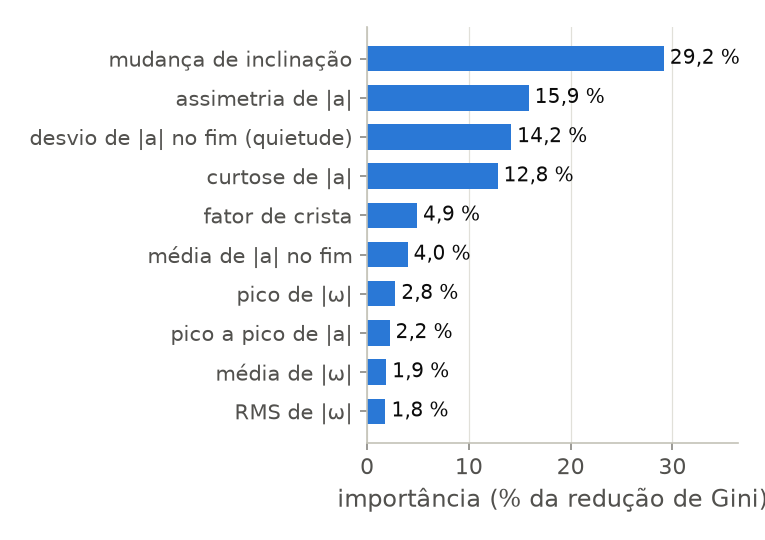
\includegraphics[width=\linewidth]{figuras/ap_importancia.png}
    \end{column}
    \begin{column}{0.4\textwidth}
      \begin{itemize}
        \item O que mais pesa é a \textbf{postura depois} (inclinação, quietude) e a \textbf{forma do impacto}
              (assimetria, curtose).
        \item O pico de $\amag$, que é o que um limiar olharia, quase não pesa.
        \item Com cada grupo de atributos sozinho, quedas com $\le$ 1 alarme/h:
          \begin{itemize}
            \item tempo: \soTempo\,\%;
            \item FFT: \soFFT\,\%;
            \item AR: \soAR\,\%.
          \end{itemize}
      \end{itemize}
    \end{column}
  \end{columns}
\end{frame}

\begin{frame}{Por que escolhemos o Random Forest}
  \centering
  {\scriptsize\begin{tabular}{@{}l rr rr r r@{}}
\toprule
 & \multicolumn{2}{c}{Alarmes falsos/h} & \multicolumn{2}{c}{Quedas com $\le$1 alarme/h} & \makecell[r]{Modelo\\na flash} & \makecell[r]{Operações\\por janela} \\
\cmidrule(lr){2-3}\cmidrule(lr){4-5}
Método & A (±8\,g) & B (±2\,g) & A & B & & \\
\midrule
\textbf{Random Forest}$^{*}$ & \textbf{0,41} & \textbf{0,76} & \textbf{95,7\,\%} & \textbf{94,4\,\%} & \textbf{252\,kB} & \textbf{46\,492} \\
SVM (RBF) & 0,76 & 0,76 & 94,6\,\% & 94,5\,\% & 45\,kB & 77\,752 \\
kNN (Manhattan) & 0,48 & 0,62 & 96,1\,\% & 96,3\,\% & 1,6\,MB & 819\,972 \\
Regressão logística & 1,44 & 1,44 & 92,8\,\% & 91,7\,\% & 412\,B & 44\,806 \\
CNN 1D (6 eixos) & 1,17 & 2,20 & 93,9\,\% & 79,4\,\% & 26\,kB & 243\,296 \\
Uma árvore só & 5,30 & 6,60 & 0,0\,\% & 0,9\,\% & 612\,B & 44\,710 \\
\bottomrule
\end{tabular}
}\\[0.05cm]
  {\tiny $^{*}$ Floresta da comparação: 150 árvores de profundidade $\le$ 12. A do vestível tem 60 árvores de
   profundidade $\le$ 10 e ocupa \rfVestKB\,kB.}\\[0.2cm]
  \begin{columns}[T,onlytextwidth]
    \begin{column}{0.49\textwidth}
      \begin{itemize}\small
        \item \textbf{Menos alarmes falsos} no cenário do vestível, com $\sim$96\,\% das quedas.
        \item \textbf{Perde pouco com a saturação} em $\pm$2\,g, que pode voltar no pulso (acima de 8\,g).
        \item \textbf{Não precisa normalizar}: cada pergunta é um limiar em g, graus ou segundos.
      \end{itemize}
    \end{column}
    \begin{column}{0.49\textwidth}
      \begin{itemize}\small
        \item \textbf{Cabe no ESP32}, com poucas comparações por janela; o custo maior é calcular os atributos.
        \item \textbf{Explicável}: mostra quais atributos pesam.
        \item O kNN guarda o treino inteiro (\knnMB\,MB), a CNN perde muito em $\pm$2\,g, e a regressão logística dá
              o triplo de alarmes.
      \end{itemize}
    \end{column}
  \end{columns}
\end{frame}

\begin{frame}{O pipeline completo, na SisFall}
  \figura{ap_funil.png}
  \vspace{-0.25cm}
  \begin{itemize}
    \item De \nEnsaiosQueda{} quedas, \funilPassam{} passam pelo gatilho, e o Random Forest reconhece
          \funilDetectadas{} (\funilDetectadasPct\,\%).
    \item Nas \horasAtividade\,h de atividades, o gatilho dispara \disparosCausal{} vezes por hora, mas sobram só
          \textbf{\rfVestAlarmes{} alarmes falsos por hora}.
  \end{itemize}
  \nota{Como roda no vestível: gatilho causal, \nAtributos{} atributos e 60 árvores; validação por pessoa.}
\end{frame}

\begin{frame}{Teste externo: os nossos \nProprios{} ensaios}
  \begin{columns}[T,onlytextwidth]
    \begin{column}{0.52\textwidth}
      \centering
      {\scriptsize\begin{tabular}{@{}l c c c@{}}
\toprule
Método & \makecell{Quedas\\detectadas} & \makecell{Alarmes\\falsos} & \makecell{Atividades\\com alarme} \\
\midrule
\textbf{Random Forest} & \textbf{7 de 10} & \textbf{0} & \textbf{0 de 8} \\
SVM (RBF) & 8 de 10 & 0 & 0 de 8 \\
Regressão logística & 7 de 10 & 0 & 0 de 8 \\
kNN (Manhattan) & 8 de 10 & 1 & 1 de 8 \\
Centroide (cosseno) & 8 de 10 & 4 & 3 de 8 \\
Regras em cascata & 8 de 10 & 5 & 4 de 8 \\
DTW & 10 de 10 & 8 & 6 de 8 \\
Correlação com templates & 10 de 10 & 12 & 6 de 8 \\
AR(12) como anomalia & 10 de 10 & 18 & 8 de 8 \\
CNN 1D & 9 de 10 & 12 & 7 de 8 \\
\bottomrule
\end{tabular}
}
    \end{column}
    \begin{column}{0.45\textwidth}
      \begin{itemize}
        \item Modelos treinados \textbf{só na SisFall} ($\pm$2\,g) e testados nos nossos ensaios, de outra pessoa e
              outro sensor.
        \item Random Forest: \textbf{nenhum alarme falso} ao andar ou correr, e todas as quedas de frente e de costas
              (\rfPropriosQuedas{} de \nPropriosQueda).
        \item Perde as quedas de joelhos: são mais lentas, e os ensaios acabam $\sim$1\,s depois do impacto.
        \item Os métodos que comparam formas detectam tudo, mas disparam em quase toda caminhada.
      \end{itemize}
    \end{column}
  \end{columns}
\end{frame}

% ============================================================
%  Vestível e próximos passos
% ============================================================
\begin{frame}{No vestível}
  \begin{columns}[T,onlytextwidth]
    \begin{column}{0.52\textwidth}
      \begin{itemize}\small
        \item \textbf{Gatilho causal}: decide amostra a amostra, sem olhar o futuro. Passam as mesmas
              \gatilhoPassam\,\% das quedas, com menos disparos (\disparosCausal{} contra \disparosPicos{} por hora).
        \item \textbf{Só os \nAtributos{} atributos no tempo}: sem FFT nem AR no C, perdendo pouco.
        \item \textbf{60 árvores de profundidade $\le$ 10}: \rfVestNos{} nós e \rfVestKB\,kB de flash;
              \rfVestAlarmes{} alarme falso/h e \rfVestSens\,\% das quedas com $\le$ 1 alarme/h.
      \end{itemize}
    \end{column}
    \begin{column}{0.46\textwidth}
      \centering
      \begin{tikzpicture}[caixa/.style={bloco, text width=2cm, minimum height=1cm}]
        \node[destaque, text width=2cm, minimum height=1cm] (v) at (0, 0) {\textbf{Vestível}\\pipeline e\\Random Forest};
        \node[caixa] (h) at (3.6, 0) {\textbf{Hub do quarto}\\ESP32-S3};
        \node[caixa] (c) at (3.6, -2.1) {\textbf{Central}\\MQTT, Grafana};
        \node[caixa, draw=queda] (t) at (0, -2.1) {\textbf{Cuidador}\\Telegram};
        \draw[seta] (v) -- node[rotulo, above] {ESP-NOW\\\texttt{FALL}} (h);
        \draw[seta] (h) -- node[rotulo, right] {alerta\\\texttt{queda}} (c);
        \draw[seta] (c) -- node[rotulo, above] {aviso} (t);
        \draw[setafina, dashed] (v.north) -- ++(0, 0.4) node[rotulo, above] {CAN \texttt{0x0FD} (bancada)};
      \end{tikzpicture}\\[0.25cm]
      \nota{A mensagem leva o pico e a $P(\text{queda})$; o alerta chega à central com o campo \texttt{prob}.}
    \end{column}
  \end{columns}
\end{frame}

\begin{frame}{Limitações e próximos passos}
  \begin{columns}[T,onlytextwidth]
    \begin{column}{0.47\textwidth}
      \textbf{\color{uspblue}Limitações}
      \begin{itemize}
        \item Todos os dados são da \textbf{cintura}; a pulseira vai no \textbf{pulso}, onde o braço se mexe muito
              mais.
        \item Os nossos ensaios: uma pessoa, curtos e saturados em $\pm$2\,g.
        \item Quedas em colchão, feitas por jovens; quedas reais de idosos são mais lentas e variadas.
      \end{itemize}
    \end{column}
    \begin{column}{0.5\textwidth}
      \textbf{\color{uspblue}Próximos passos}
      \begin{enumerate}
        \item Gravar o firmware e conferir o pipeline na bancada: custo em ciclos e decisões.
        \item \textbf{Coletar no pulso}, em $\pm$8\,g, com várias pessoas e ensaios mais longos.
        \item Retreinar o modelo e rever o gatilho com esses dados. O script gera o modelo em C e os testes de
              paridade juntos.
      \end{enumerate}
    \end{column}
  \end{columns}
\end{frame}

\begin{frame}[plain]
  \centering
  \vspace{3.2cm}
  {\Huge\bfseries\color{uspblue} Obrigado}
\end{frame}

\end{document}
